%% 美赛模板:正文部分

\documentclass[12pt]{article}  % 官方要求字号不小于 12 号,此处选择 12 号字体
\usepackage{float}
\usepackage{graphicx}
\usepackage{caption}
\usepackage{subcaption}
\usepackage{listings}
\usepackage{xcolor}
% 本模板不需要填写年份,以当前电脑时间自动生成
% 请在以下的方括号中填写队伍控制号
\usepackage[2021054]{easymcm}  % 载入 EasyMCM 模板文件
\problem{C}  % 请在此处填写题号
\usepackage{mathptmx}  % 这是 Times 字体,中规中矩 
%\usepackage{mathpazo}  % 这是 COMAP 官方杂志采用的更好看的 Palatino 字体,可替代以上的 mathptmx 宏包

\title{Past Tells a Lot:\\Indicators and Predictive Models for Future Market Reaction}  % 标题

% 如需要修改题头(默认为 MCM/ICM),请使用以下命令(此处修改为 MCM)
%\renewcommand{\contest}{MCM}

% 文档开始
\begin{document}

% 此处填写摘要内容
\begin{abstract}
  In recent years, online shopping has become a new fashion. Retailers have realized it and started to pay more attention to the online market.
Before we started analyzing the sales records of the Sunshine Company, we quantified the emotional and the rational tendency of the reviews, set up two prerequisite measures called \textbf{Polarity} and \textbf{Subjectivity}.
Firstly, we designed indicators by Bootstrapping to measure the effectiveness of a review. We defined our \textbf{Trust Indicator $T$} to sieve out trustworthy combinations of ratings and reviews. Then we established the\textbf{ Effectiveness Indicator $E_{ff}$} by reconciling the length of comments, $T$, and the Subjectivity to tell if a comment is useful.
Secondly, we studied the interaction between ratings. By creating virtual customers to fit the actual rating records, we discovered a pattern which suggests the clustering effect of rating in a specific period. We named it \textbf{Interactive Rating Model}, and it helps company realize the importance of their reputation.
Finally, we used our “virtual customers” to predict future ratings based on the data we already had. Our prediction showed the consistency of the clustering effect. It enlightens companies that even avoiding a succession of negative ratings can help promote future market feedbacks.
It is also worth mentioning that we managed to ensure the stability of our indicators and models, making them generally adaptive. Since we implemented object-oriented programming, we can simply just feed in new data when needed to study new products, and our codes will solve the rest.

    % 美赛论文中无需注明关键字。若您一定要使用,
    % 请将以下两行的注释号 '%' 去除,以使其生效
    % \vspace{5pt}
    % \textbf{Keywords}: MATLAB, mathematics, LaTeX.

\end{abstract}

\maketitle  % 生成 Summary Sheet
\tableofcontents  % 生成目录


% 正文开始
\section{Introduction}
\subsection{Problem Background}
With the advance of technology and the Internet revolution, shopping online is becoming a major trend for youngsters. Different from shopping offline, online shopping has advantages. For shoppers, they are exposed to various types of products, then have more choice when buying a product. But this caused the competition between vendors much fiercer than ever. Since customer can neither feel and touch the product, nor can they see them in naked eyes, the customers' ratings and comments on shopping platforms such as Amazon influence the customer to purchase or not directly. The success or failure of a product, is greatly determined by the reviews and ratings from the customers.
\newline

\noindent
Five major problems are discussed in this paper, which are:
\begin{itemize}
    \item How to determine whether a review or rating is informative for the company to track.
    \item How will the ratings and comments influence the customers' view of product.
    \item Ways to identify a potentially successful product.
    \item Defining time-based measures that might suggest whether a product's reputation is increasing or decreasing.
    \item In what way is the star rating the customer gave relates with his comments.
      
      
\end{itemize}


\subsection{Our work}
\begin{enumerate}[\bfseries 1.]
    \item We used machine learning to analyze the emotions of customer's comments.
    \item We used object-oriented programming to objectify customers and products.
      \item We found out how previous reviews and ratings of a product may influence a customer to rate.
    \item We simulated the process of customers rating products.
    \item We developed a time-based measure that might suggest a product's reputation is increasing or decreasing.
      \item We defined a method to measure the effectiveness of a customer's comment.
\end{enumerate}

\section{Notations}
The primary notations used in this paper are listed in Table \ref{tb:notation}.
\begin{table}[H]
\begin{center}
\caption{Notations}
\begin{tabular}{cl}
	\toprule
	\multicolumn{1}{m{3cm}}{\centering Symbol}
	&\multicolumn{1}{m{12cm}}{Definition}\\
	\midrule
  $P_{ol}$&Indicator of the Polarity of a comment\\

$S_{ub}$&Indicator of the Subjectivity of a comment\\

$L_{w}$&Actual quantity of words in a comment\\

$l_{w}$&Relative quantity of words in a comment\\

${R}$&Rating of a product\\

$d$&1-D Euclidian Distance between $P_{ol}$ and the corresponding rating ${R}$\\

$d_{n}$&Normalized d by applying margin scaling method\\

$T$&The identity between $P_{ol}$ of a comment and the corresponding rating ${R}$\\

  $E_{ff}$&Effectiveness of a rating-comment combination\\
  $R_{epu}$&Indicator of product reputation\\

$t$&Time increment measured by days since the earliest date\\

$P_{ol\_hist}(t)$&Indicator of historical polarity until day $t$\\

$T_{hist}(t)$&Indicator of historical $T$ until day $t$\\

$R_{hist}(t)$&Indicator of historical rating until day $t$\\

$R_{epu\_hist}(t)$&Indicator of historical reputation until day $t$\\

$S(t)$&Quantity of all items on a dataset before day $t$\\
	\bottomrule
\end{tabular}\label{tb:notation}
\end{center}
\end{table}

\section{The Models}

\subsection{The Effectiveness of a customer's comment}

\subsubsection{Basic assumptions}

To analyze comments, ratings combined with other data, traditionally we can simply use supervised learning algorithms, however, it would require clear labels for each combination in the dataset. Without labels, we must first find a way to understand the information lies within texts, and MOST importantly, extract indicative, quantitative measures for further analysis.

​		From our daily language usage, it is not hard to find that emotional words have a kind of polarity from negative to positive. And more interestingly, similar emotional word tend to cluster. Although emotional transition do exist, it would be easy to distinguish by acknowledge some conjunctions and commas.

​		Moreover, when people are expressing strongly subjective willing, the frequency of using "I" and other emotional words would increase, suggesting that we can tell the subjectivity from contexts.

​		With these two features, it enlightens us that, quantified polarity and subjectivity indicators for each comment could be highly valuable, as shopping comments are basically combinations of customers' emotional expresses and rational analysis of products.

\subsubsection{Extractions from comments}

\label{sec:Extractions from comments}

With the assumptions above, we should first find ways to extract the Polarity $P$ and the subjectivity $S$.

​		We acknowledge that there are mature NLP (Natural Language Processing) techniques and multiple Python add-ons have been written. And we choose \textbf{TextBlob} as our analyzing tool. In this tool, it would calculate a Word Vector Space and measure these words automatically and give them a polarity value and a subjectivity value in $[0,1]$. We make sums of both measures in every comment, and get our $P$ and $S$ in each dataset.

​		But $P$ and $S$ are not the indicators we desire, as they vary a lot by the length of a comment. Therefore, we calculate the quantities of words for each comment, noted as $L_{w}$. And get our average $P_{avg}$ and $S_{avg}$ as follows:
$$
P_{avg} = \frac{P}{L_{w}}
\quad\quad
S_{avg} = \frac{S}{L_{W}}
$$
​		As  $P_{avg}$, $S_{avg}$ and $L_{w}$ are all logistic values, we normalize them to $[0,1]$, and note them as $P_{ol}$,  $S_{ub}$ and $l_{w}$ in each dataset. The normalization method is as follows:
$$
l_{w} = \frac{L_{w} - \mathrm{MIN}(L_{w})}{\mathrm{MAX}(L_{w}) - \mathrm{MIN}(L_{w})}
$$

$$
P_{ol} = \frac{P_{avg} - \mathrm{MIN}(P_{avg})}{\mathrm{MAX}(P_{avg}) - \mathrm{MIN}(P_{avg})}
\quad\quad
S_{ub} = \frac{S_{avg} - \mathrm{MIN}(S_{avg})}{\mathrm{MAX}(S_{avg}) - \mathrm{MIN}(S_{avg})}
$$

​		Note that $R$ can have only five values in $\{1,2,3,4,5\}$, we also normalize it to make it coincide with other measures, meaning $R$ in the following analyzing process can only take values in $\{0,0.25,0.5,0.75,1\}$

​		The preprocessing of our datasets is complete.

\subsubsection{Trust Indicator}

​		The rating-comment system provides both a general summary of experience and detailed textual information. But sometimes people can have inconsistency when making it. For example, there are 5-star ratings combined with less flattering words, maybe out of good will. Some would say "can be better" or "just so-so", but also gave a 5-star. Sometimes the system just records a default comment "five stars", both situations can result in low $P_{ol}$ value but high rating $R$.

​		To solve this problem, we need to design a "Trust Indicator" $T$, to sieve out those inconsistent combinations of ratings and comments. To reach the definition, we first define some supportive measures.

​		One of our teammate got inspired by the sigmoid function by his previous learning of Machine Learning, as it serves quite well when doing the logistic regression problem. The sigmoid function is as follows:
$$
\mathrm{Sigmoid}(x) = \frac{1}{1+\mathrm{e}^{-x}}
$$


​		Sigmoid function has a very good features, it maps $R$ to $(0,1)$, and because it climbs fast near 0, it has the tendency to classify data on $R$ into two separate parts, 0 or 1. Therefore, sigmoid function would be perfect for us to tell if a data is trustworthy or not.

​		But we still need to consider what it should be the "$x$" of the $Sigmoid(x)$. As described above, the $P_{ol}$ shows the emotional preference of a comment, therefore the inconsistency can be described by $P_{ol}$ and $R$. We define the 1D-Euclidian distance $d$ as:
$$
d = \vert P_{ol} - R\vert
$$
​		Directly fit "$d$" as our "$x$" is clearly not a good idea, as an ideal $x$ should fit on $R$. To reach a good classification performance, we should map our $d$ to $R$ before we send our $x$ into the function. Here we choose $tan(x)$. Practical calculation shows that $d$ usually not fit the range $[0,1]$ perfectly, they close to each other a bit, so we apply the same normalization method as we have done in the preprocessing. In each dataset, we take $d_{n}$ as the normalized $d$:
$$
d_{n} = \frac{d - \mathrm{MIN}(d)}{\mathrm{MAX}(d) - \mathrm{MIN}(d)}
$$
​		Then we map $d_{n}$ to $R$, result noted as $t(d_{n})$:
$$
t(d_{n}) =k \tan(\pi  (0.5-d_{n}))
$$
​		Now we get $t(d_{n})$ as our desired "$x$", and we send it into $Sigmoid(x)$, considering the edge points, we can define our $T$ as follows:
$$
{T} = \left\{\begin{matrix}
1 &d=0\\ 
\frac{1}{1+\mathrm{e}^{-t(d_{n})}} & 0<d<1\\ 
0 & d=1
\end{matrix}\right.
$$
​		To be specific, $k$ is a positive constant to adjust how fast it can be when the curve climbs as our $d_{n}$ is near 0.5. If $k$ is too large, few points get a middle middle value of $T$; otherwise we reach a bad classification performance, which we would not desire. The $T-d_{n}$ relation graph is as follows:

\begin{figure}[H]
  \centering
  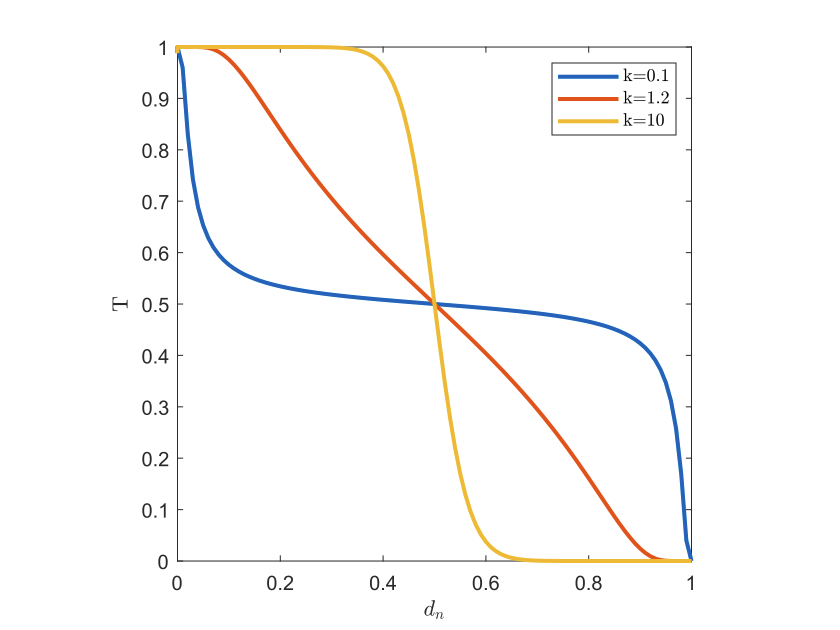
\includegraphics[width=0.7\linewidth]{Q1picture/Q1dnT.png}
  \caption{The $T - P_{ol}$ Graph}
  \label{fig:}
\end{figure}


​		By testing for multiple times, we find choosing $k$ in $(1,2)$ can reach a balance between the diversity of $T$ and classification performance.

\subsubsection{Evaluation of the Trust Indicator}


​		We plot the $T - P_{ol}$ Graph as follows:
\begin{figure}[H]
  \centering
  \includegraphics[width=0.7\linewidth]{Q1picture/T-pol.jpg}
  \caption{The $T - P_{ol}$ Graph}
  \label{fig:}
\end{figure}


​		For products with lower ratings, our $T$ increases as  $P_{ol}$ drop, and vice versa for those with higher ratings. For middle-rated products to have higher $T$, because the average $P_{ol}$ is around 0.4, and 1 \& 2 star correspond to 0.25 \& 0.5 in normalized $R$, which naturally result in smaller $d$. 

​		Although this property means $T$ cannot serve as perfect indicator of whether a comment can be trusted, it is still needed for further analysis, as it weakens comments with extreme ratings, specifically 5-Star and 1-Star, helping us pick out really useful comments.

​		When $k = 1.2$, about 12\% of all the data we have satisfies $T > 0.8$.

\subsubsection{Effectiveness Indicator}




​		When we are shopping online, some comments of a relatively longer length with objective descriptions could sometimes inspire or wave our willing. Although voting on comments can indicate whether they are useful or not, it does not work when a new product just come online. Moreover, voting can be faked or can simply be an expression of emotion. Therefore, voting can be referable, but not reliable.

​		Since we already have $T$, we should use it along with other data we have to design a much more reliable indicator to help us find effective comments.

​		Relating to our daily life, we think a effective comment should be:

- With sufficient textual information
- Mostly objective
- Trustworthy

​		Relatively seen, some comments are much longer than the others, we would also like to see comments of medium size which can provide us useful information. We define our Effectiveness Indicator as $E_{ff}$:
$$
E_{ff}=(1-S_{ub}) \times \sqrt{l_{w}}\times T
$$
​		We tested this by looking at the top 100 comments with the highest $E_{ff}$, useful comments with or without votes both appeared in our view, meaning this indicator do can help us pick out effective comments.



\subsection{Statistics on a timeline}

​		To talk about this problem, we first need to define what a timeline is on each dataset. Considering the variance of data, we cannot assure that the earliest items of all three datasets take place on the same day. Therefore we use relative increment to represent the shift of time.

​		On a specific dataset, we take $D_{current}$ as the current date and $D_{earliest}$ as the earliest date in the dataset, then we define the time increment $t$ as follows:
$$
t = D_{current} - D_{earliest}
$$
​		This is easy to calculate on a modern computer as date is also stored as time increment since Jan. 1st, 1970.

​		With a timeline, we can define some useful statistical indicators based on days:
$$
P_{ol\_hist}(t) = \frac{\sum_{0}^{t} P_{ol}}{S(t)}
$$

$$
T_{hist}(t) = \frac{\sum_{0}^{t} T}{S(t)}
$$

$$
R_{hist}(t) = \frac{\sum_{0}^{t} R}{S(t)}
$$

​		We use the pacifier dataset to calculate indicators above, then plot the $P_{ol\_hist}(t)-t$ and the $R_{hist}(t)-t$ graph here:

​		Note that in both graphs, $t$ is normalized.
\begin{figure}[H]
  \centering
  \begin{subfigure}{.5\textwidth}
    \centering
    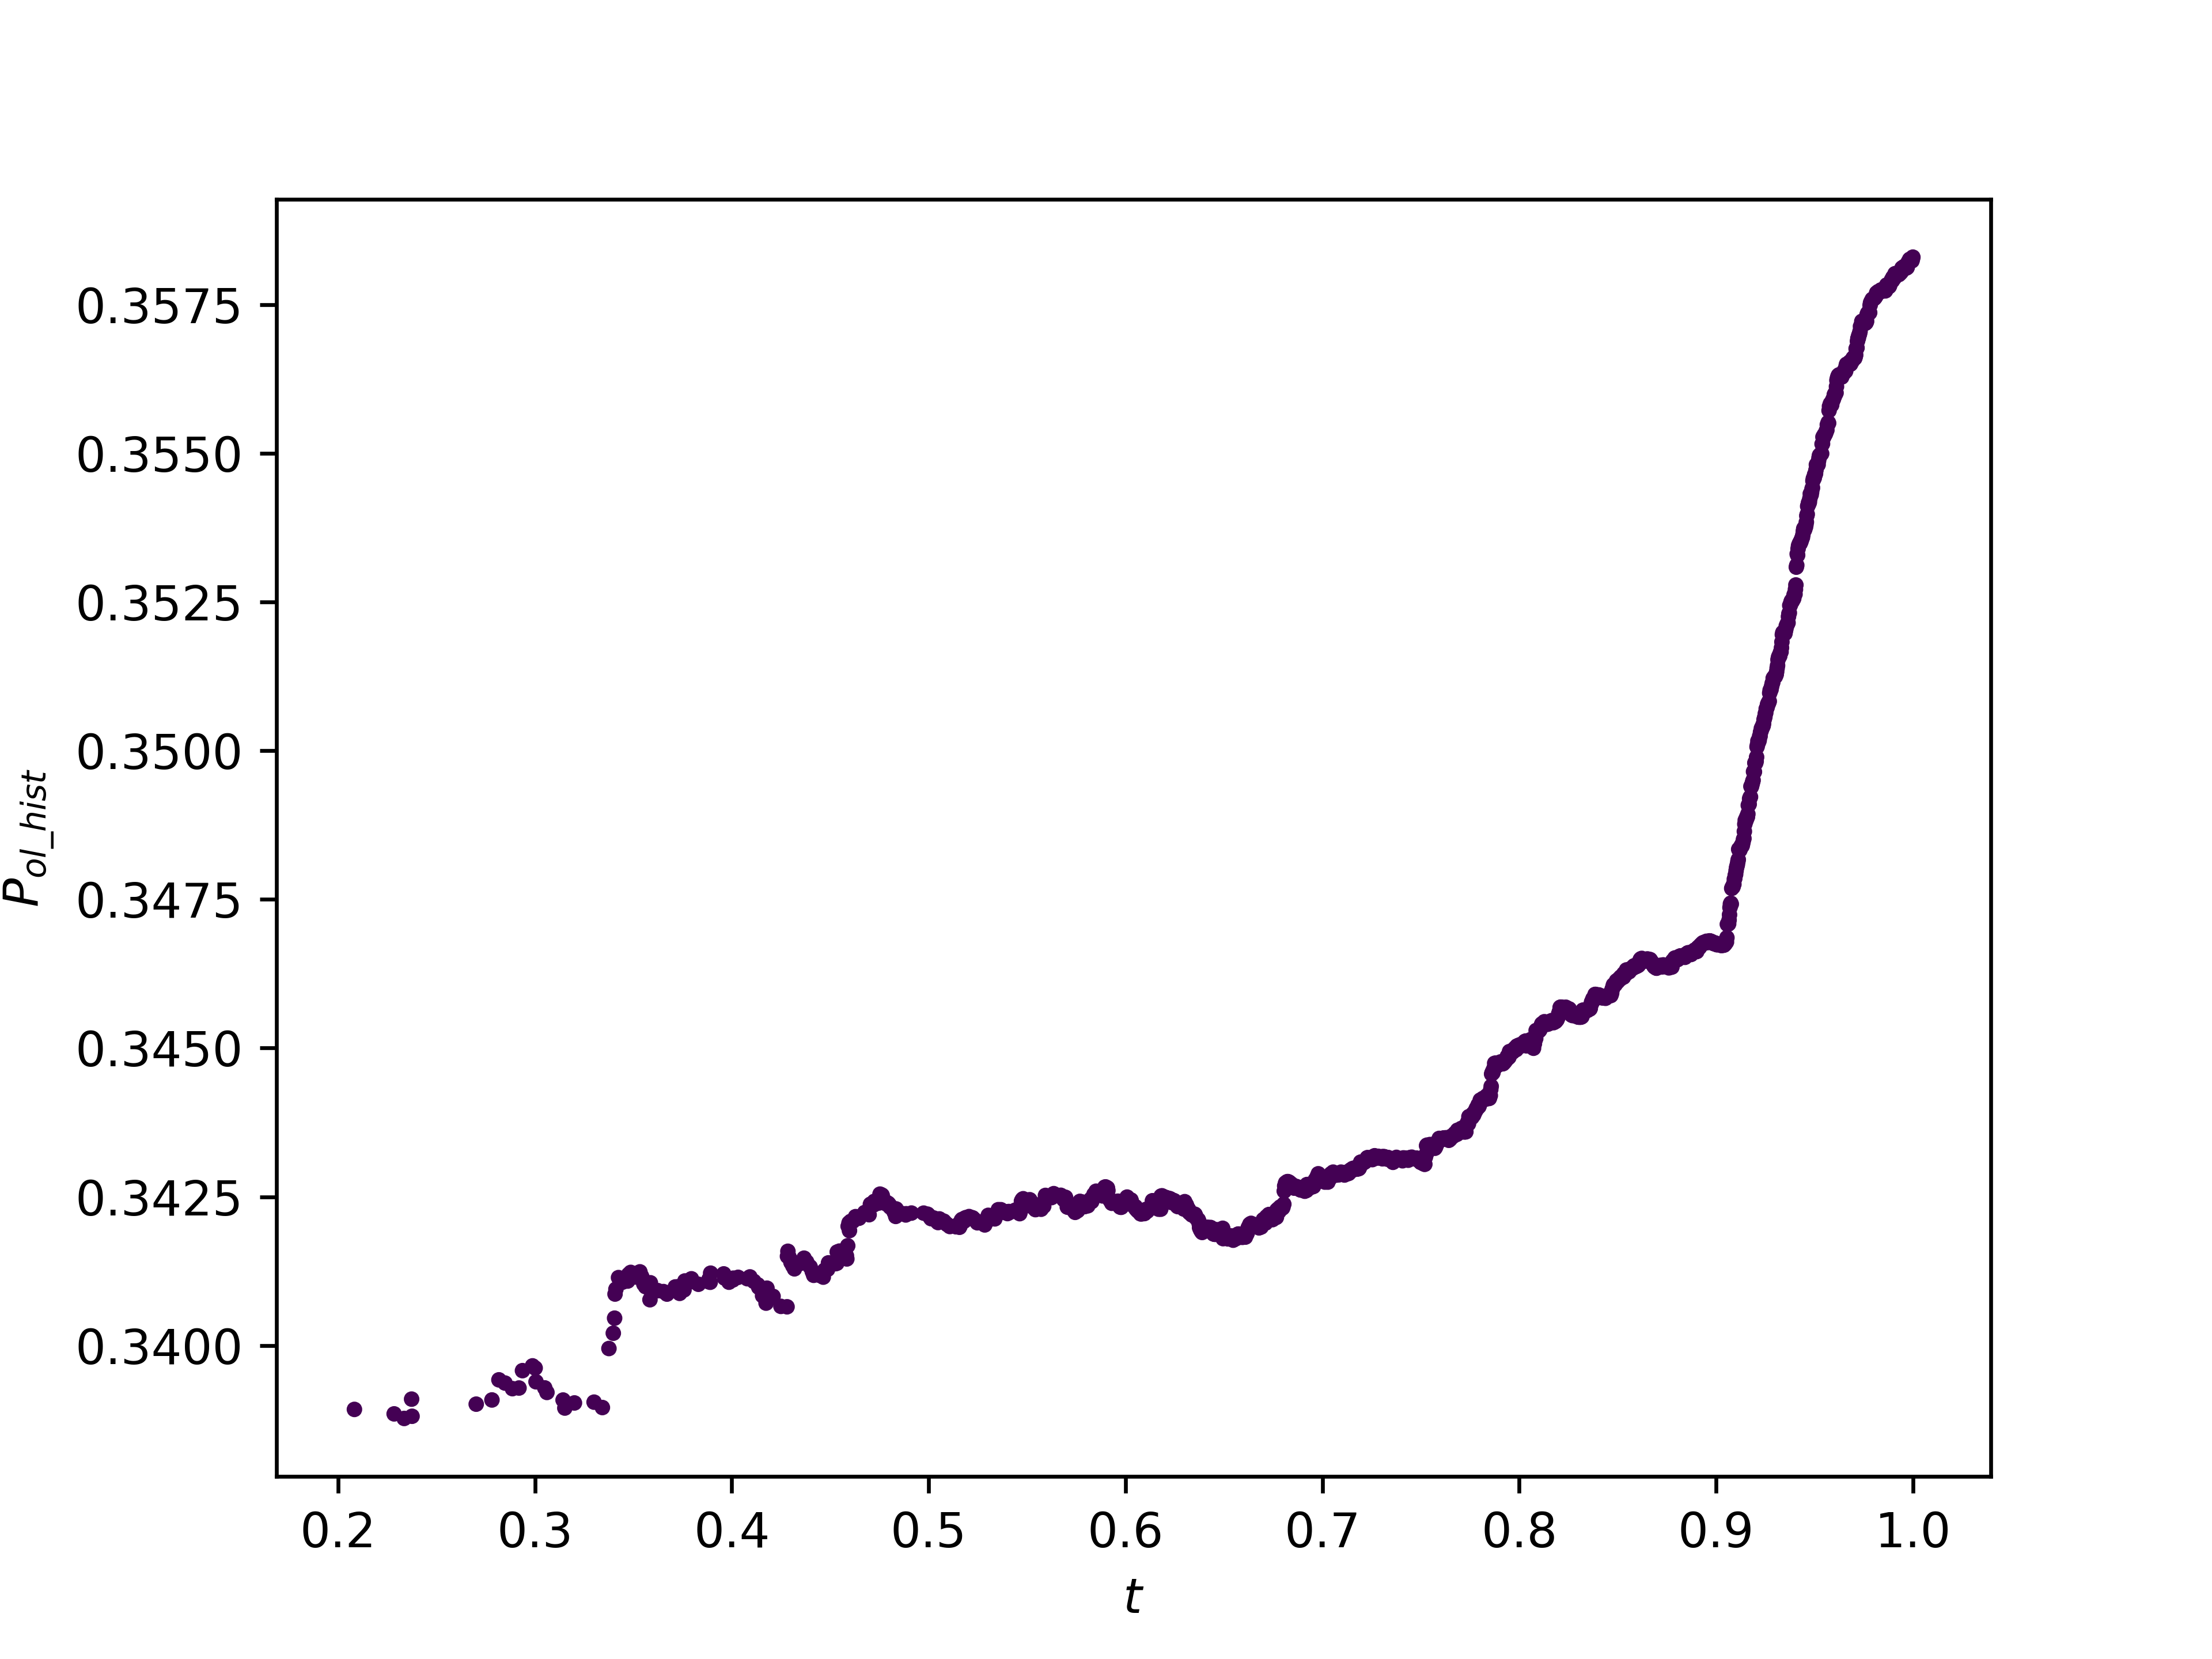
\includegraphics[width=\linewidth]{Q2picture/Pol_hist-t.png}
    \label{fig:}
  \end{subfigure}%
  \begin{subfigure}{.5\textwidth}
    \centering
    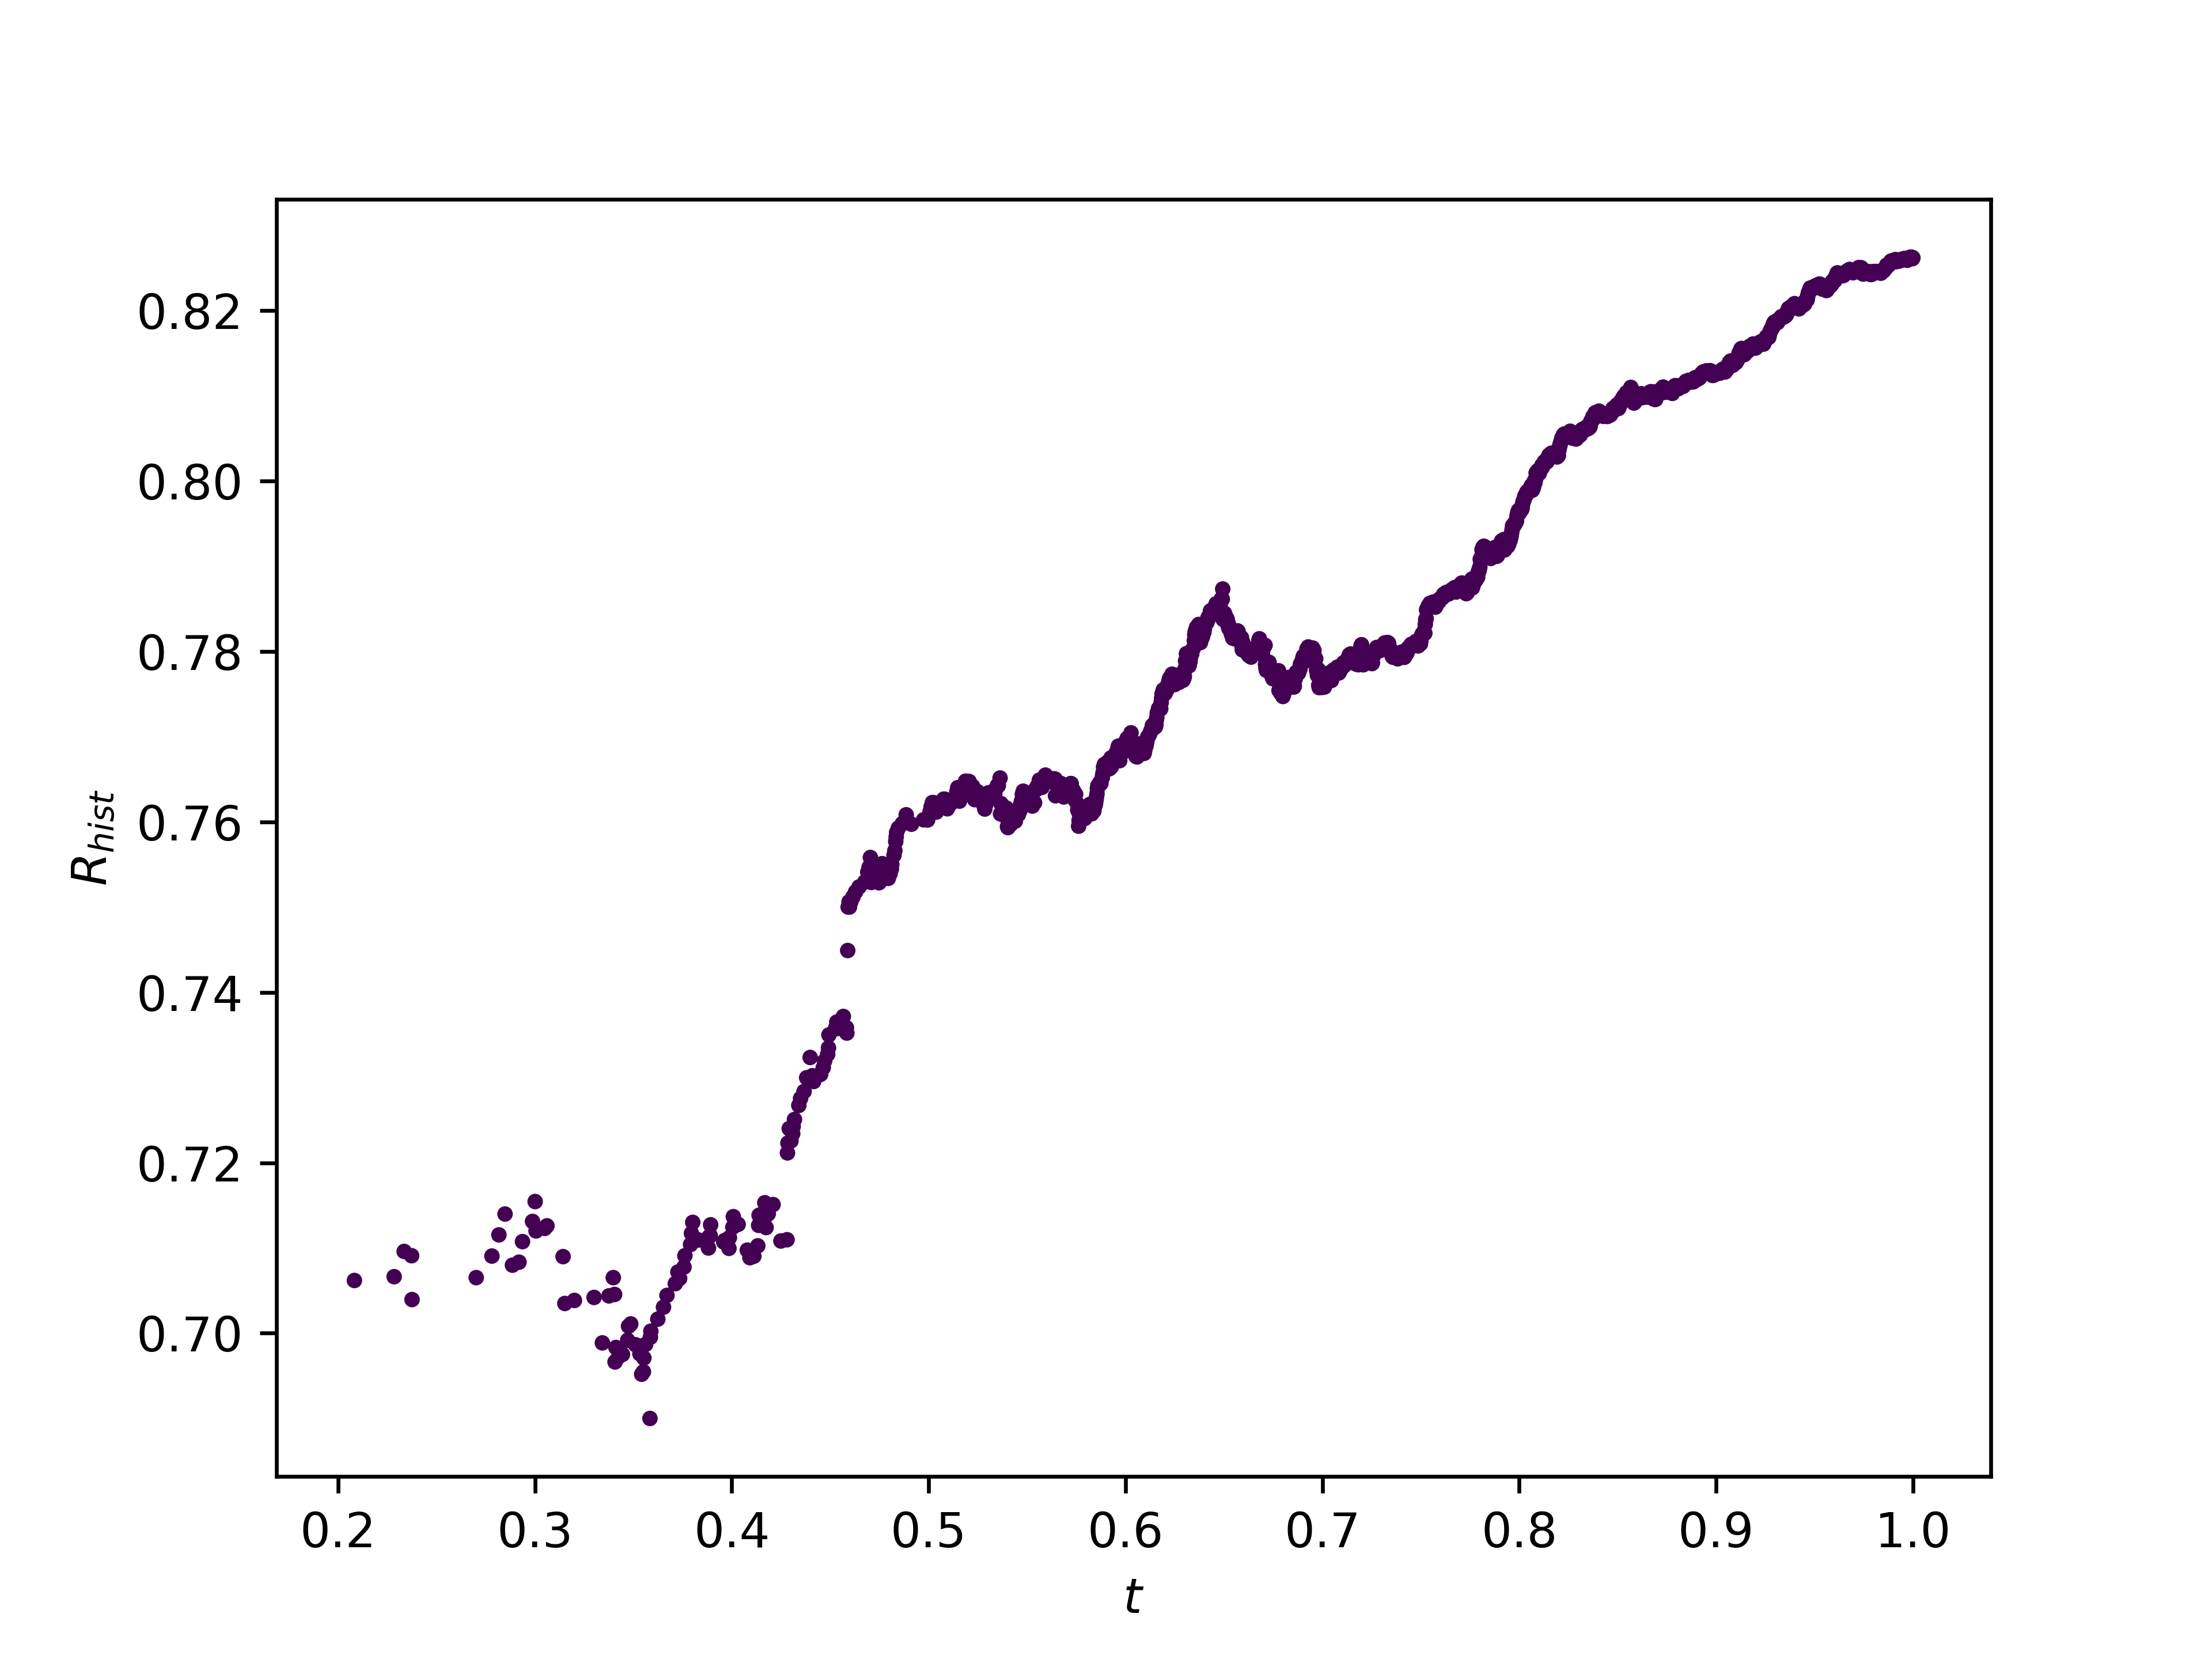
\includegraphics[width=\linewidth]{Q2picture/R_hist-t.png}
    \label{fig:}
  \end{subfigure}
  \caption{the $P_{ol\_hist}(t)-t$ and the $R_{hist}(t)-t$ graph}
  \label{fig:}
\end{figure}


​		Turning points are very important because we may potentially find useful information, like the adjustments made to advertising, to products and so on; however, we may notice turning points in one graph vary from those in another. Therefore we start to think about the necessity of a new indicator which reconciles both two important indicators about customers' experience.

​		We call it Reputation Indicator, noted as $R_{epu}$. We used the weakening feature of $T$ to lower the impact of $P_{ol}$ on our $R_{epu}$.
$$
R_{epu} = T \times P_{ol} + R
$$
​		And correspondingly, we have its historical average:
$$
R_{epu\_hist}(t) = \frac{\sum_{0}^{t} R_{epu}}{S(t)}
$$
​		We plot the $T_{hist}(t)-t$ and the $R_{epu\_hist}(t)-t$ graph on the pacifier dataset as follow:

​		Note that in both graphs, $t$ is normalized.
\begin{figure}[H]
  \centering
  \begin{subfigure}{.5\textwidth}
    \centering
    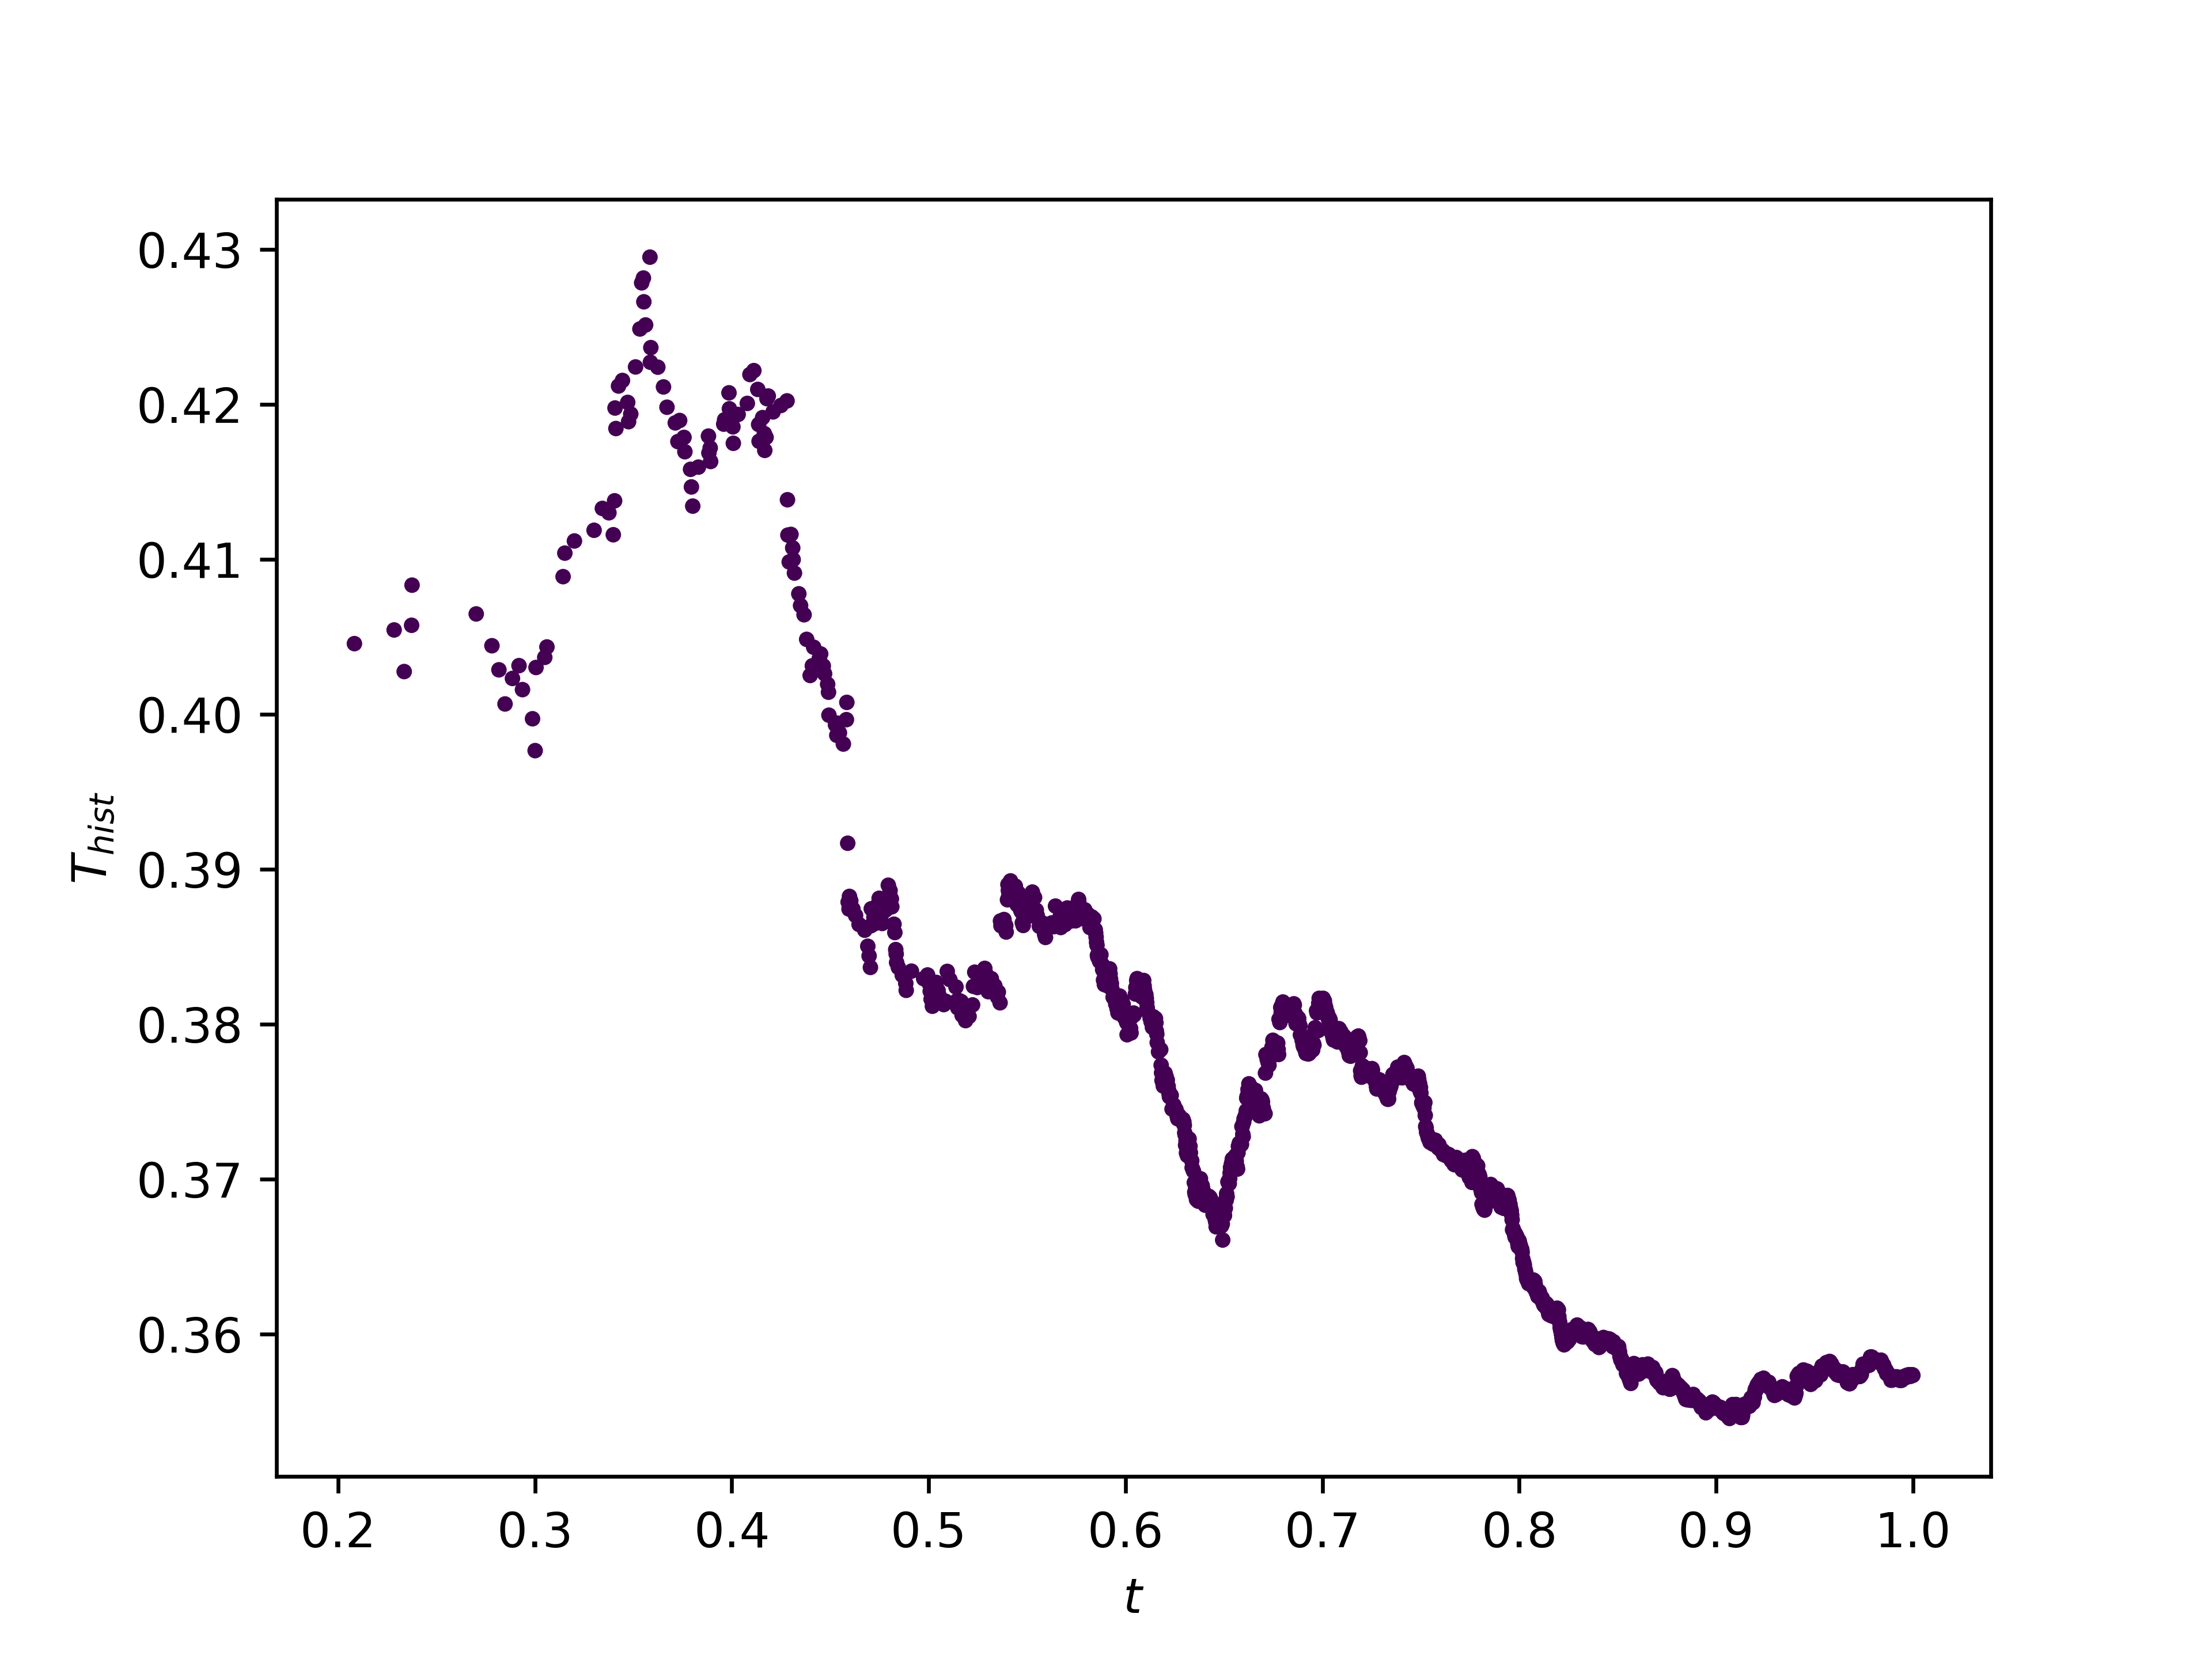
\includegraphics[width=\linewidth]{Q2picture/T_hist-t.png}
    \label{fig:}
  \end{subfigure}%
  \begin{subfigure}{.5\textwidth}
    \centering
    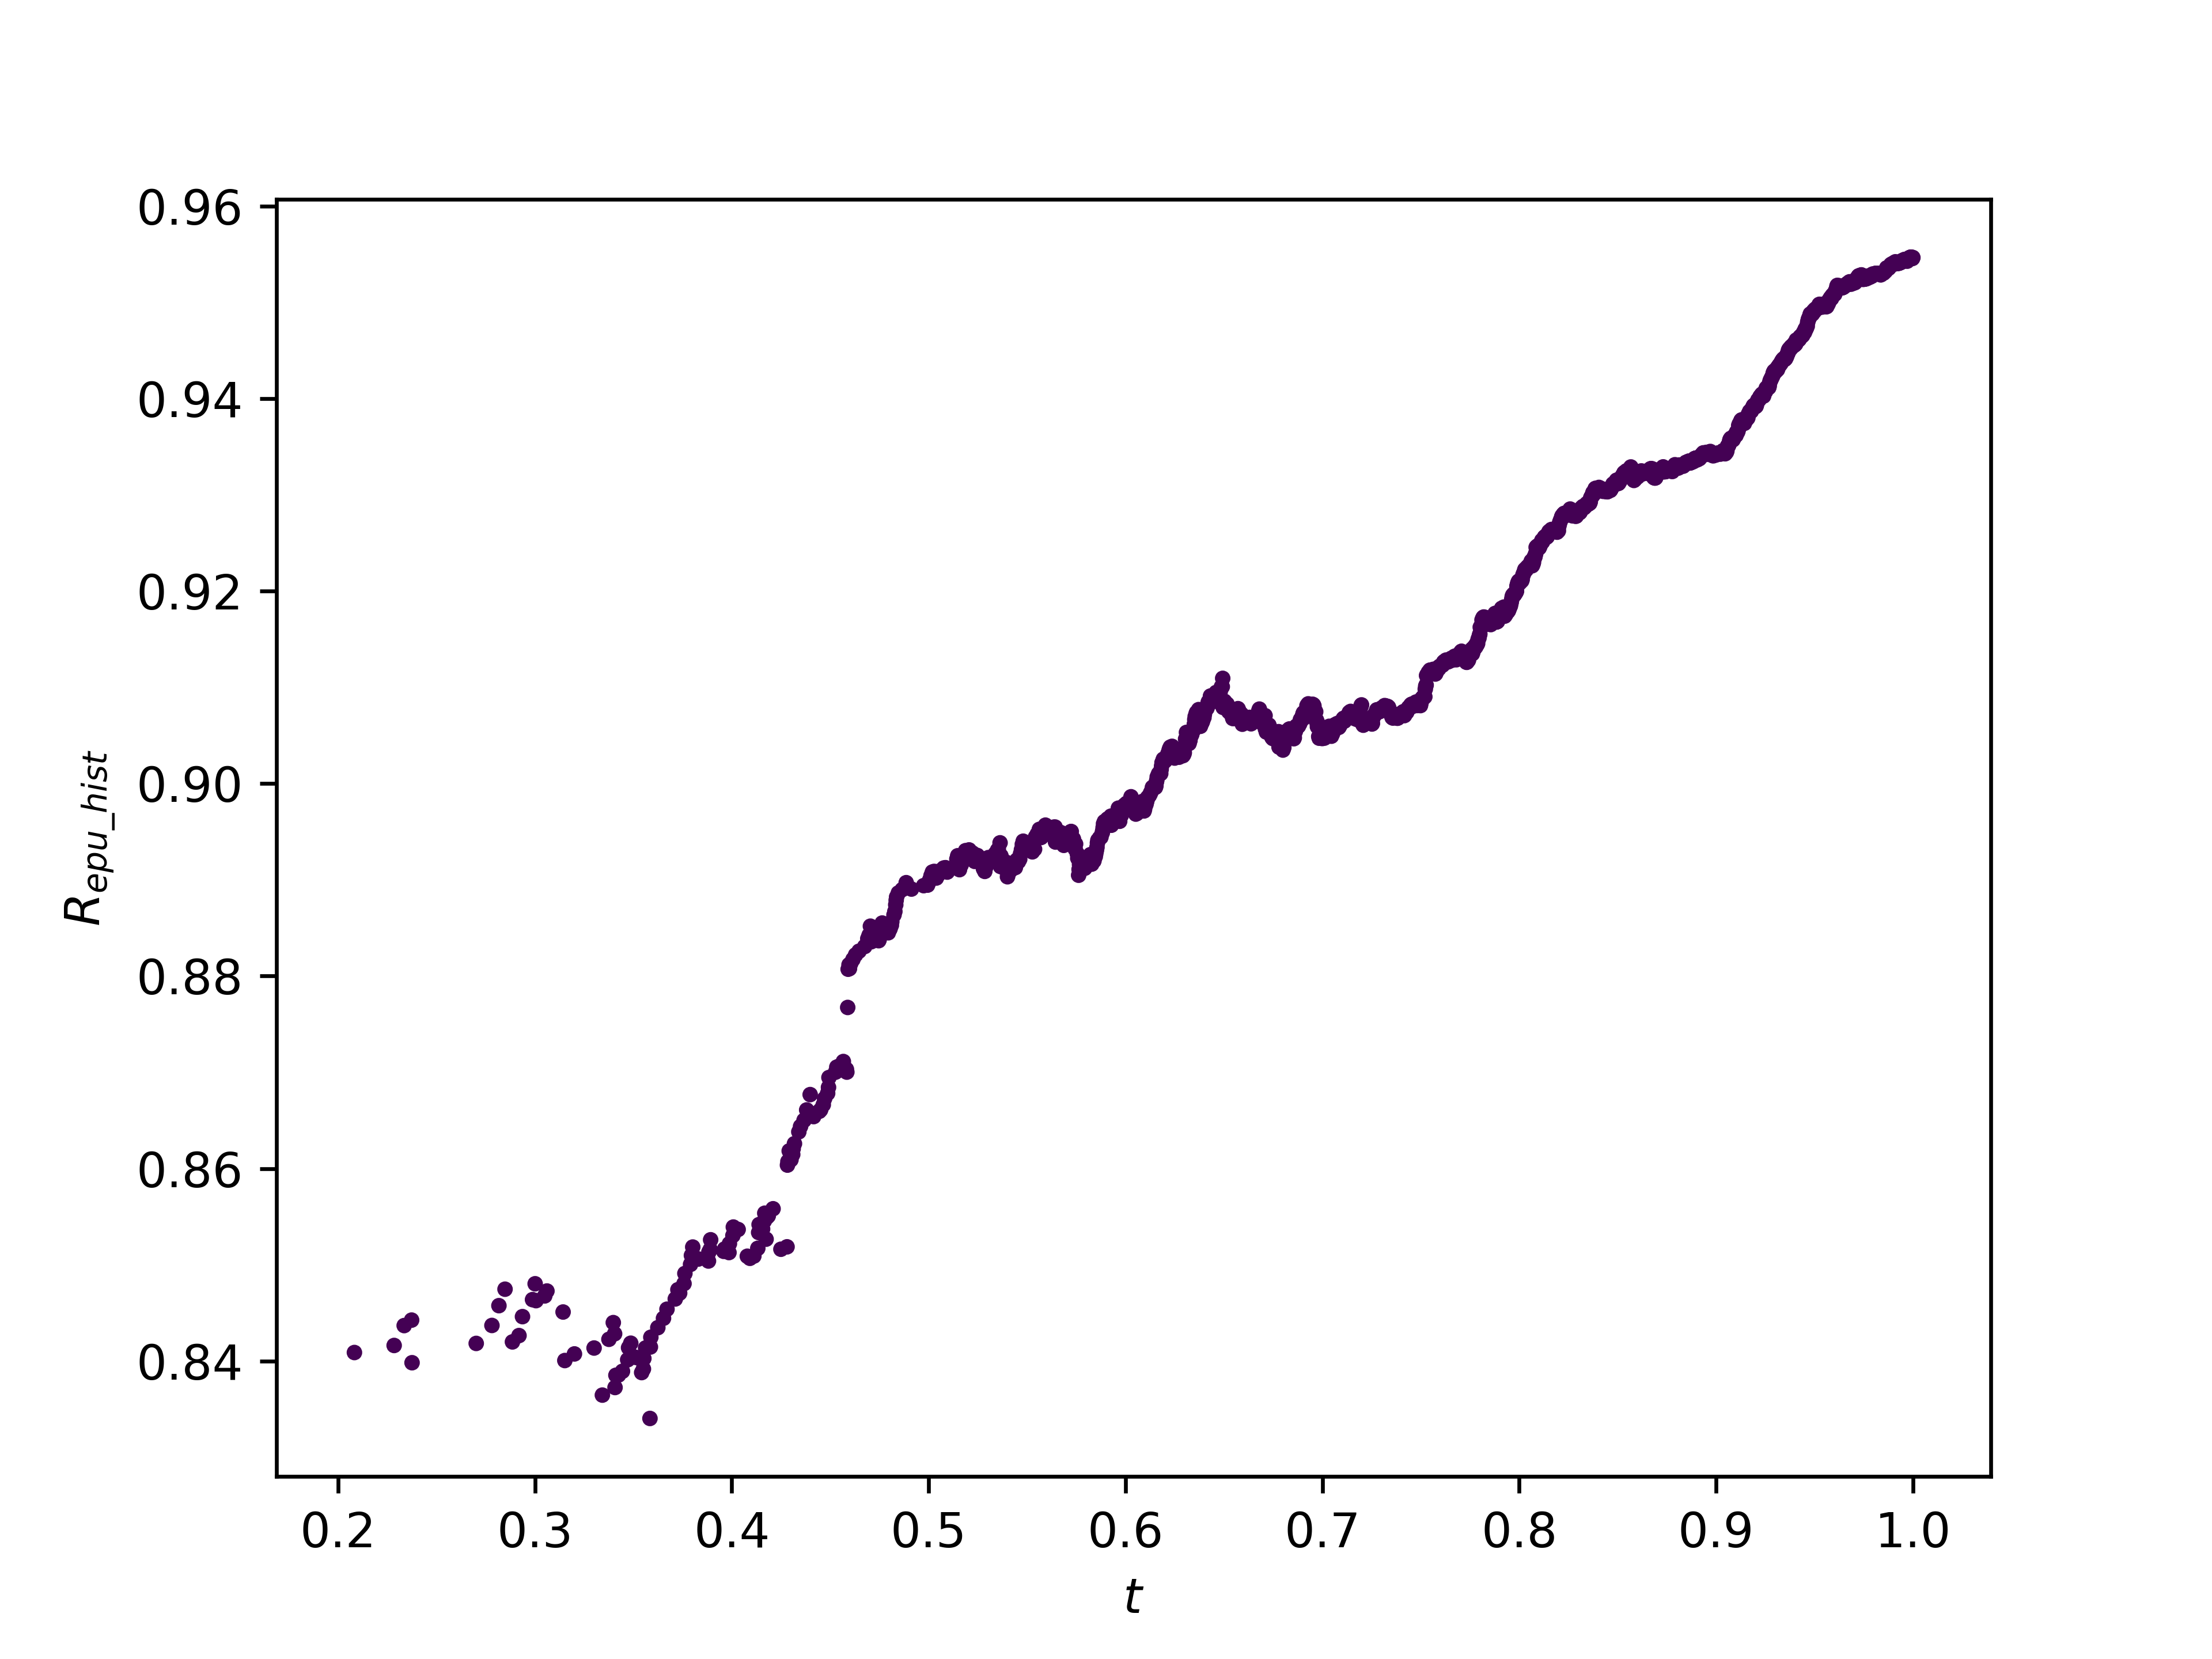
\includegraphics[width=\linewidth]{Q2picture/Repu_hist-t.png}
    \label{fig:}
  \end{subfigure}
  \caption{the $T_{hist}(t)-t$ and the $R_{epu\_hist}(t)-t$ graph}
  \label{fig:}
\end{figure}


​		From approximately $t = 0.45$, when the data points got denser since then, $T$ slightly drops from 0.39 to lower than 0.36. However, our $R_{epu\_hist}(t)$ still remained the increasing trend, meaning it making obvious progress on the pacifier product.

​		Talking about the turning points in the $R_{epu\_hist}(t)-t$ graph, it is noticeable that the turning points of the TWO graphs above mostly appeared on this one, though we have a more smoothly increasing curve.

% \subsection{The subjectivity and polarity of a customer's review}
% We assumed that each word, in the customers' reviews, has 2 properties: \textbf{subjectivity} and \textbf{polarity}. Subjective $s_{word}$ describes in what degree the word is subjective, ranges from 0 to 1. The higher $s_{word}$ is, the more subjective a word is. Polarity $p_{word}$ describes how much the customer loves or hates the product when writing the word, ranges from -1 to 1. We then define the subjectivity and the polarity of a sentences $s_{sentence}$ and $p_{sentence}$, which is the average of all the words in a sentences. Assume the number of words in a sentence is $n$, then
% \begin{equation*}
%   \begin{aligned}
%     s_{sentence} = \dfrac{\sum\limits_{n} s_{word}}{n}  \\
%     p_{sentence} = \dfrac{\sum\limits_{n} p_{word}}{n} 
%   \end{aligned}
% \end{equation*}
% Apparently, if a customer A used 1 sentence to praise a product, and customer B used 10 sentences to praise it, customer B loves it more. So we sum up all the subjectivity and polarity of the sentences in customer's review, to indicate how subjective the customer is, and in what degree the customer loves or hates the product.
% \begin{equation*}
%   \begin{aligned}
%     s_{customer} = \sum s_{sentence} \\
%     p_{customer} = \sum p_{sentence}
%   \end{aligned}
% \end{equation*}
% To solve this problem, of course we need a word list to store the subjectivity and polarity of different words. Perhaps we need machine learning. But in solving this problem, we didn't reinvent wheels because the wheel we invented probably won't better than the wheels in open source communities. So we used \textbf{textblob} , a python module, to calculate the subjectivity and polarity of the customers.

\subsection{The relation between rating levels and customer reviews}

To find the relation between rating levels and customer reviews, first we need to convert customer reviews, which is text based information, to numeric numbers. As we said in section \ref{sec:Extractions from comments}, we calculated the subjectivity and polarity of each customer, according to their reviews. And we used the \textbf{Curve Fitting} app in \textbf{MATLAB}, trying to fit a curve.
We imported the subjectivity, polarity and star ratings data of all the 3 products separately into \textbf{MATLAB}, and plotted the data. Then we could see from the graph that the polarity seemed to be linearly dependent with star rating, and the polarity is not dependent with star rating.
Then we used Linear Method to fit the data. These following graphs shows the relation between polarity, subjectivity and star rating of the 3 different products.
\begin{figure}[H]
  \centering
  \begin{subfigure}{.5\textwidth}
    \centering
    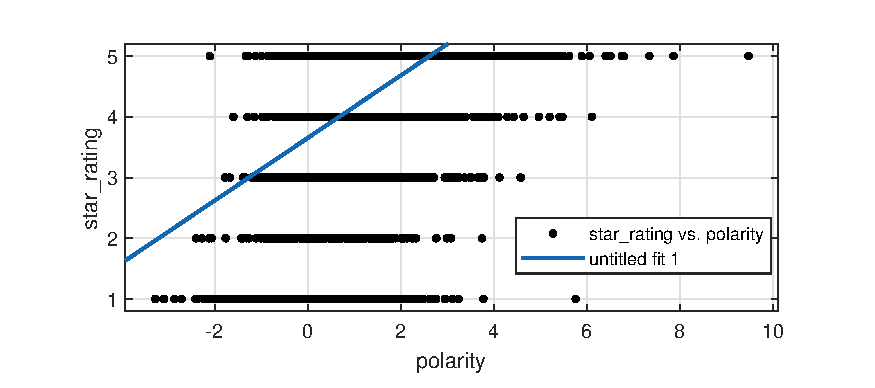
\includegraphics[width=\linewidth]{figures/hair_dryer/polarity_vs_star_rating.eps}
    \caption{star rating vs polarity}
    \label{fig:}
  \end{subfigure}%
  \begin{subfigure}{.5\textwidth}
    \centering
    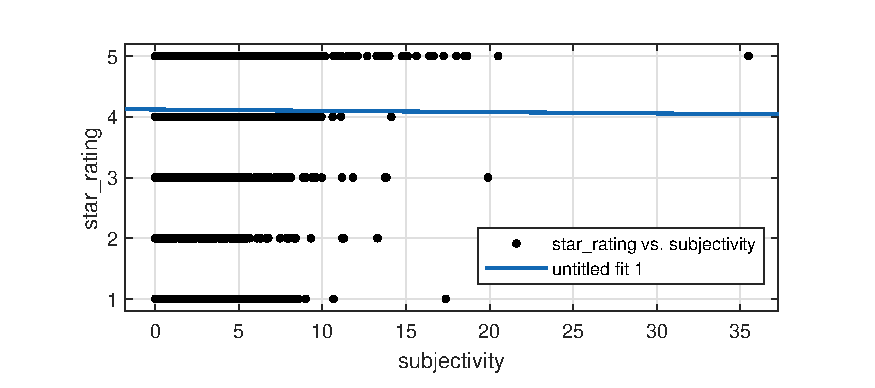
\includegraphics[width=\linewidth]{figures/hair_dryer/subjectivity_vs_star_rating.eps}
    \caption{star rating vs subjectivity}
    \label{fig:}
  \end{subfigure}
  \caption{the relation between polarity, subjectivity and star rating of the hair dryer}
  \label{fig:}
\end{figure}
\begin{figure}[H]
  \centering
  \begin{subfigure}{.5\textwidth}
    \centering
    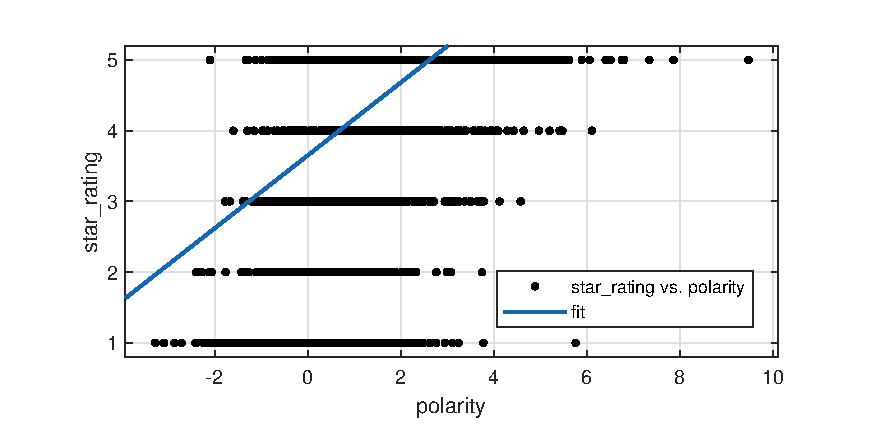
\includegraphics[width=\linewidth]{figures/microwave/polarity_vs_star_rating.eps}
    \caption{star rating vs polarity}
    \label{fig:}
  \end{subfigure}%
  \begin{subfigure}{.5\textwidth}
    \centering
    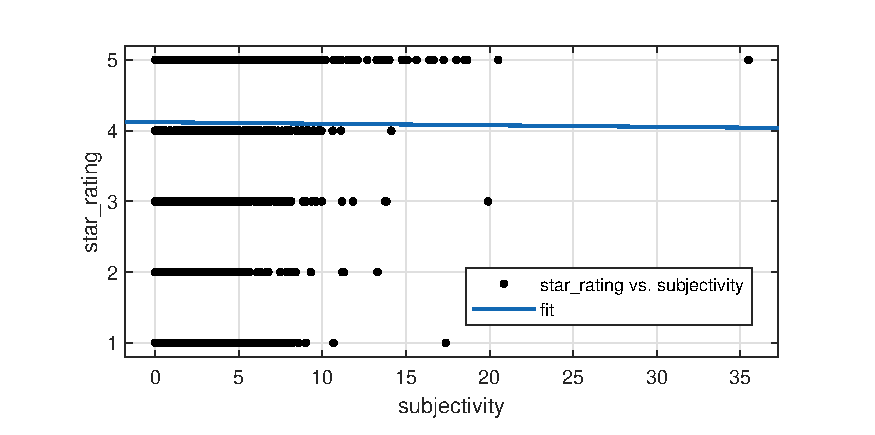
\includegraphics[width=\linewidth]{figures/microwave/subjectivity_vs_star_rating.eps}
    \caption{star rating vs subjectivity}
    \label{fig:}
  \end{subfigure}
  \caption{the relation between polarity, subjectivity and star rating of the microwave}
  \label{fig:}
\end{figure}
\begin{figure}[H]
  \centering
  \begin{subfigure}{.5\textwidth}
    \centering
    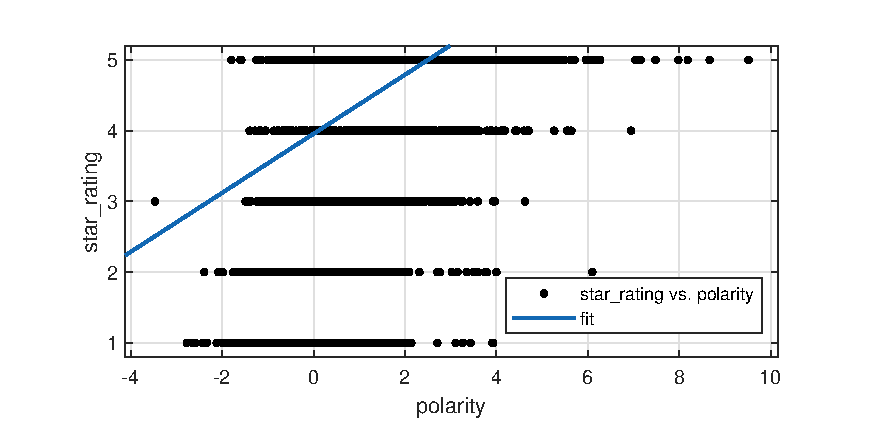
\includegraphics[width=\linewidth]{figures/pacifier/polarity_vs_star_rating.eps}
    \caption{star rating vs polarity}
    \label{fig:}
  \end{subfigure}%
  \begin{subfigure}{.5\textwidth}
    \centering
    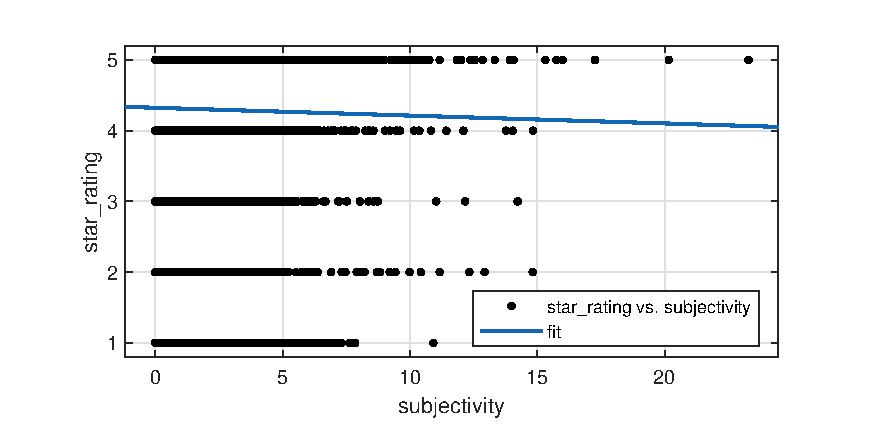
\includegraphics[width=\linewidth]{figures/pacifier/subjectivity_vs_star_rating.eps}
    \caption{star rating vs subjectivity}
    \label{fig:}
  \end{subfigure}
  \caption{the relation between polarity, subjectivity and star rating of the pacifier}
  \label{fig:}
\end{figure}
As \textbf{MATLAB} told us, the star rating, noted in $R$, is linearly related with customer's polarity $P_{ol}$. And $R$ is unrelated with subjectivity of the customer $S_{ub}$. For the hair dryer
\begin{equation*}
  \begin{aligned}
    R = 0.515 P_{ol} + 3.652
  \end{aligned}
\end{equation*}
For the microwave
\begin{equation*}
  \begin{aligned}
    R = 0.5949 P_{ol} + 2.969
  \end{aligned}
\end{equation*}
For the pacifier
\begin{equation*}
  \begin{aligned}
    R = 0.4172 P_{ol} + 3.957
  \end{aligned}
\end{equation*}

\subsection{The influence among different star ratings and reviews}
\label{sec:The influence among different star ratings and reviews}

For customers, writing reviews and rating products are commonly not completely an individual behavior. For instance, if you see others giving bad comments to a product, you will tend to think that the product is not as good as the product it actually is. In finding how previous reviews and star ratings may infect a customer's view of a product, we made the following assumptions

\begin{enumerate}[\bfseries 1.]
\item Assume that the customer is only infected by previous reviews and star ratings. Customers may not be infected by the vendors, the shopping platforms, etc. The final star rating is decided by the customer's experience and other's ratings.
\item Assume that the customer is more convinced by the reviews whose star rating is close to his own star rating.
\item Assume the customer tend to read from the latest reviews rather than reviews far previous.
\item Assume the number of reviews a customer tends to see obeys normal distribution, and the average reviews a customer wants to see is 5. So that the user won't see a review which is created, for example, 1 year ago. When the reviews are created doesn't matter in this problem.
\end{enumerate}

According to the first 2 assumptions, we define the influence, to determine in what degree others' reviews may effect a customer's review. Because the reviews is linearly related with the star rating, we use star rating to represent the customers' attitude towards the product. We define
\begin{equation*}
  \begin{aligned}
    I = k_1 (R - \bar{R}) + k_2 (R - \bar{R}_{star})
  \end{aligned}
\end{equation*}
Whereas $I$ is the influence, $R$ is the star rating customer tend to give before seeing others reviews, $\bar{R}$ is the average star rating of product before the user gives a rating, which indicates the quality of a product at that time. $\bar{R}_{star}$ is the average of star rating the customer seen, $k_1$ and $k_2$ are constants.

We used object-oriented programming of \textbf{MATLAB} to solve the problem. The source code of the program is in \textbf{Appendix}

In the program, we defined 2 classes: Customer and Product. Customers has properties like polarity and subjectivity, and product has reviews given by customers. We created the same amount of customers given by the data, set $k_1$ and $k_2$ to different values, then set the polarity and subjectivity of the created customers to the real customers' polarity and subjectivity. And let them to give star ratings of the product one by one in order.

Each customer will see random amount of previous reviews, and the star rating a customer finally give in the stars he may give before seeing the reviews plus the influence $I$

We carefully adjust the 2 constants, until the distribution of star ratings those customers gave is similar to the real star ratings in data.

We used the data of hair dryer. When we set $k_1=0.7$ and $k_2=0.13$, we found the data we manually created was quite similar with the real one. The following graph shows the distribution of star ratings and the difference between the real data and the data we created.

\begin{figure}[H]
  \centering
  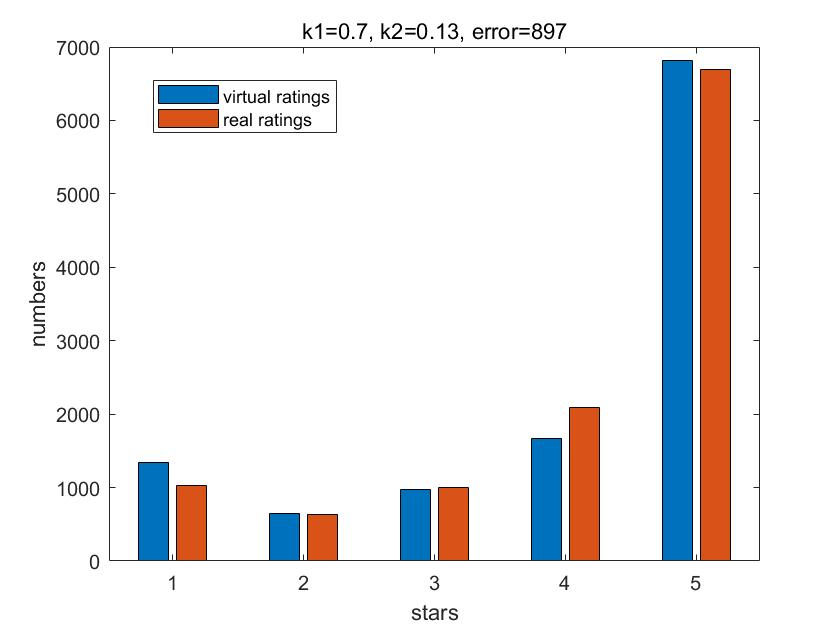
\includegraphics[width=0.7\linewidth]{Q4picture/0.jpg}
  \caption{The distribution of star ratings of hair dryer}
  \label{fig:}
\end{figure}

Since the customers see random numbers of previous reviews and star ratings, to show our model is stable, we ran the program for 2 more times. And the outputs are almost the same.

\begin{figure}[H]
  \centering
  \begin{subfigure}{.5\textwidth}
    \centering
    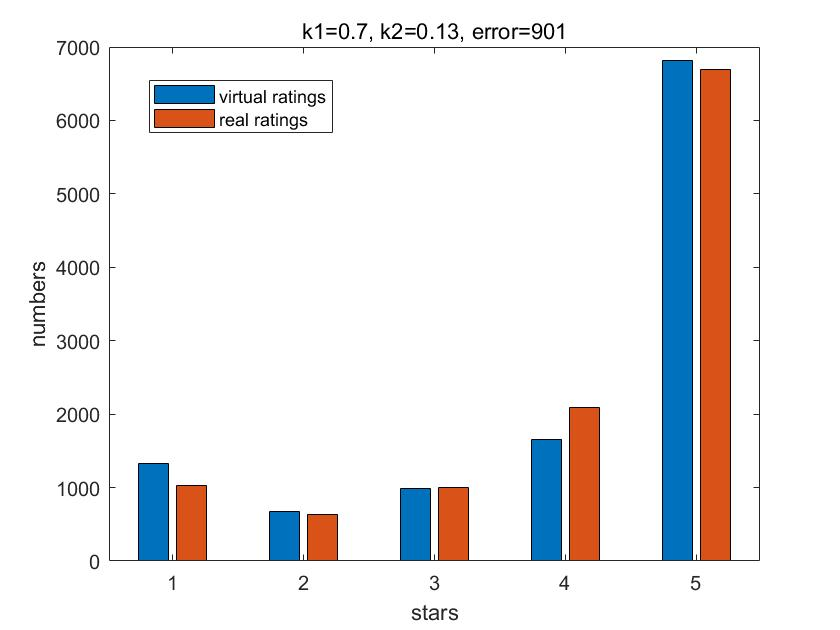
\includegraphics[width=\linewidth]{Q4picture/1.jpg}
    \label{fig:}
  \end{subfigure}%
  \begin{subfigure}{.5\textwidth}
    \centering
    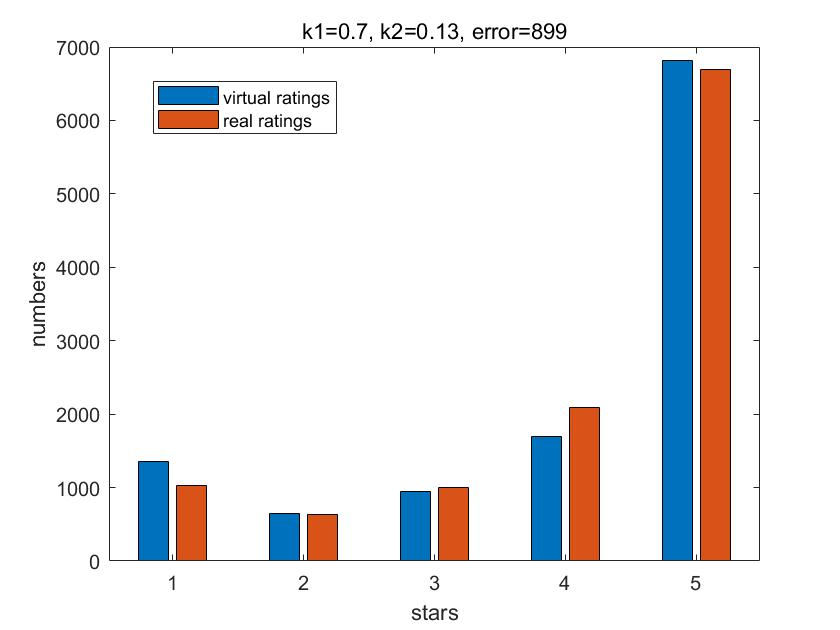
\includegraphics[width=\linewidth]{Q4picture/2.jpg}
    \label{fig:}
  \end{subfigure}
  \caption{The program gave us same result each time we ran}
  \label{fig:}
\end{figure}

Then we applied the same model to the pacifier and the microwave, and , surprisingly, we founded out that for different products, the 2 constants, $k_1$ and $k_2$, are the same.

That is probably because the 2 constants are properties of customers, and are not related to certain products, and the customers are the same. These 2 graphs show that our model fixed well on the microwave and pacifier as well.


\begin{figure}[H]
  \centering
  \begin{subfigure}{.5\textwidth}
    \centering
    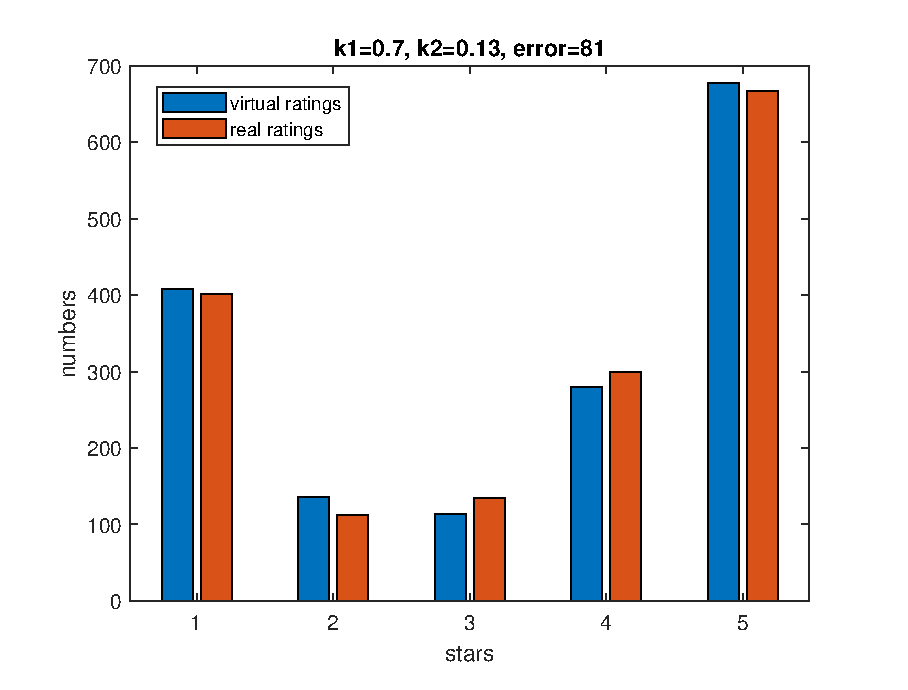
\includegraphics[width=\linewidth]{Q4picture/microwave}
    \caption{The distribution of star ratings of microwave}
    \label{fig:}
  \end{subfigure}%
  \begin{subfigure}{.5\textwidth}
    \centering
    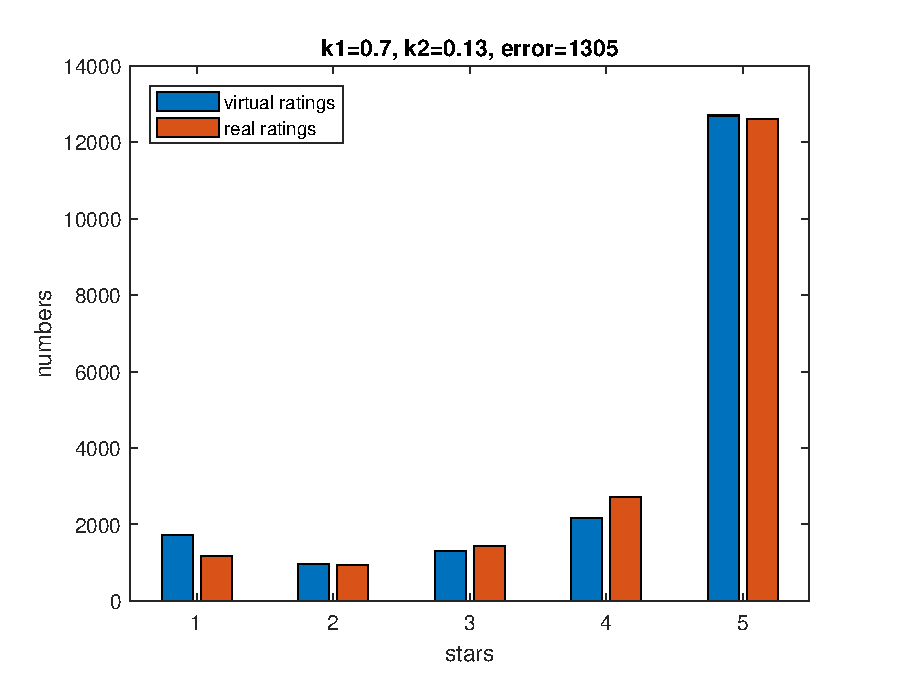
\includegraphics[width=\linewidth]{Q4picture/pacifier}
    \caption{The distribution of star ratings of pacifier}
    \label{fig:}
  \end{subfigure}
  \caption{Our model fits well on other products}
  \label{fig:}
\end{figure}

\subsection{Predict the future of the 3 products}

Since the data of star rating we created can successfully fit the real star ratings of all the 3 products, if we create more customers, we can predict their ratings as well.

Our assumptions is the same as before. And to ensure the future customers is the same as the customers we had known from data, we assume the polarity and subjectivity obey normal distribution.

We used the \textbf{Distribution Fitter} app in \textbf{MATLAB} to find the $\sigma$ and $\mu$ of the normal distribution polarity and subjectivity obeys. And we created future customers, whose polarity and subjectivity is generated from the 2 normal distribution we just known.

The rating customers gave before being influenced by other reviews are linearly dependent with their polarity. And the relation is already known in section \ref{sec:The influence among different star ratings and reviews}

For the hair dryers and the pacifier, we created 5000 future customers, and the distribution of their ratings are shown below

\begin{figure}[H]
  \centering
  \begin{subfigure}{.5\textwidth}
    \centering
    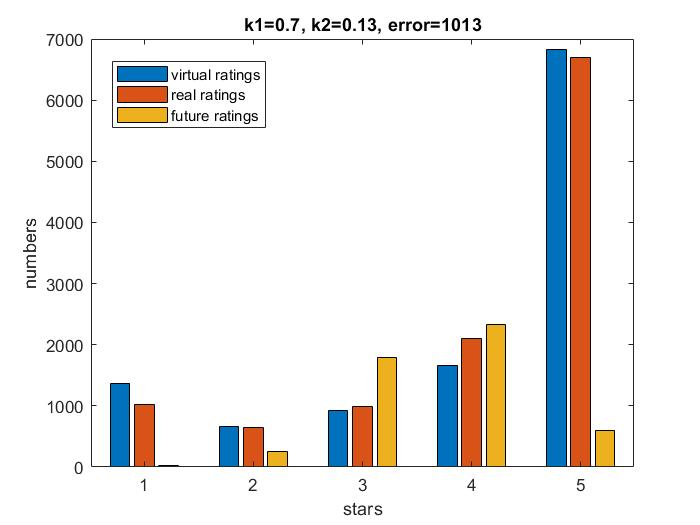
\includegraphics[width=\linewidth]{Q3picture/hair_dryer.jpg}
    \caption{The distribution of star ratings of hair dryer}
    \label{fig:}
  \end{subfigure}%
  \begin{subfigure}{.5\textwidth}
    \centering
    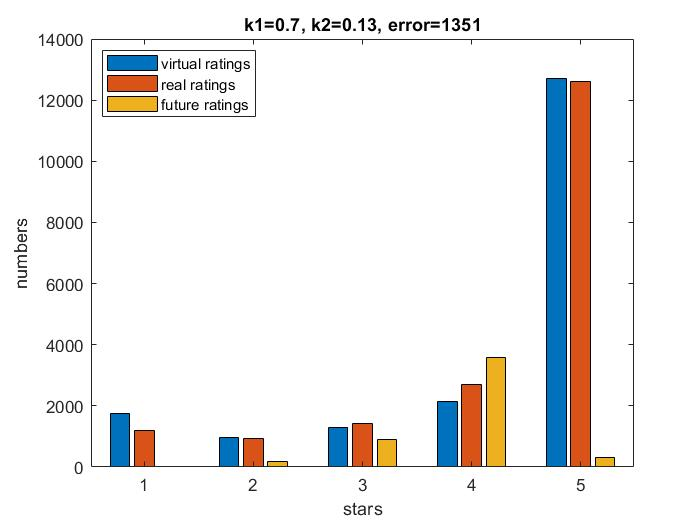
\includegraphics[width=\linewidth]{Q3picture/pacifier.jpg}
    \caption{The distribution of star ratings of pacifier}
    \label{fig:}
  \end{subfigure}
  \caption{The future star ratings our model predicted}
  \label{fig:}
\end{figure}

We can see that future customers tend to give 4 stars, and the reputation of the 2 products may stay unchanged.

But for the microwave, we created 500 future customers, and found out the future customers spoke highly of the microwave, compared to the customers we known from data. Less 1 star ratings are generated, more high star ratings appeared. This indicates that the microwave may has potential to success.
\begin{figure}[H]
  \centering
  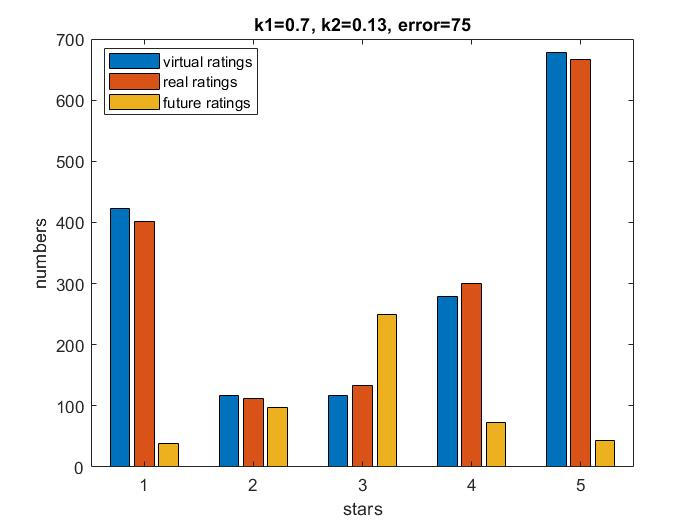
\includegraphics[width=0.7\linewidth]{Q3picture/microwave.jpg}
  \caption{The future star ratings of microwave we predicted}
  \label{fig:}
\end{figure}



\section{Strengths and Weaknesses}
\subsection{Strengths}
\begin{itemize}
\item We used object-oriented programming, which means that our models are extensible and easy to understand. For example, if you need to edit the behavior of customer, you may just edit the customer class, add some functions or properties into it.
  \item We took random factors into our consideration. For example, the customers see random amount of previous ratings, the properties of our created future customers is random.
  \item The simulated data our model outputs fits the real data quite well.
    \item The 2 constants, $k_1$ and $k_{2}$, is not related to products. So our model can be applied to other products.
\end{itemize}

\subsection{Weaknesses}
\begin{itemize}
    \item The customers' polarity and subjectivity seem not obeying normal distribution. Perhaps they obey Blotzmann distribution, or perhaps we should generate future customers whose polarity and subjectivity has the same frequency as real customers, and let them to rate products in random orders. We are disappointed at this failure in modeling, but the deadline doesn't await.
 \end{itemize}


% 以下为信件/备忘录部分,不需要可自行去掉
% 如有需要可将整个 letter 环境移动到文章开头或中间
% 请在后一个花括号内填写信件(Letter)或备忘录(Memorandum)标题
 \begin{letter}{A Letter to the CMO of Sunshine Company}
   \noindent
   \textbf{\Large A Good Reputation Makes Things Perfect}
   
\noindent
Dear CMO of the Sunshine Company,

​I would like to extend my most sincere greetings to you.

​We are honored to be your consultant team to assist you analyzing the marketing data of your company, hoping to find potentially successful business models and to provide constructive advice. After struggling for four days, we have completed our analysis, and we are very delighted to share our insights with you.

​Starting from the measurement of the comment effectiveness, we based our work on it and developed a set of methods to show how reviews affect each other and to predict short-term market reactions. Here is what we want you to know:

\noindent
\textbf{We ​found a model that can extract highly informative comments.}

    We proposed our Trust \& Effectiveness indicators, showing that middle-rated, moderately lengthy, and objective comments tend to be most useful. And we verified our proposition by listing out those comments we believe useful. Please take a look at them with our methods.

\noindent
\textbf{We proposed a model revealing how rating impact each other to predict the future reputation.}
    
    According to the data, we find previous ratings may affect the future ones. We proposed a model to predict future sales trend by measuring and fitting interactions between ratings. By our modeling, we noticed that new ratings tend to cluster. The actual rating of consumers is not only determined by their consumption experience, but also affected by pervious rating, the gap between new rating and total star rating, or the recent rating gap. And the greater the gap, the greater the effects will be.

\noindent
\textbf{We analyzed the sales status of the product.}
    
By creating hundreds of people, virtually reading previous reviews, we found that bad ratings close to the present one may result in the dropping of the future reputation, and customer impression as well. Take the example of the microwaves, recent negative comments would make future trend of rating to stay low, even if the essence of your product has never changed.

​Overall, we would like you to read less about accusation but longer and more objective comments. Accusation sometimes can only be accusation itself, but comments with customers' analysis would be mostly sincere and informative. Also, never underestimate the impact of your business reputation’s influence ability, previous reviews stand for it. It hardly fades away and would impact on your future sales. A better after-sale service may help you avoid continuous bad comments.

​We wish you prosperous.

\begin{flushright}
 Sincerely,

Team \#2021054

\end{flushright}
\end{letter}


% 参考文献,此处以 MLA 引用格式为例
\begin{thebibliography}{99}
\bibitem{1} MATLAB Documentation - MathWorks, from\url{https://www.mathworks.com/help/matlab/}
\bibitem{2} TextBlob: Simplified Text Processing, from\url{https://textblob.readthedocs.io/en/dev/}
\bibitem{3} Matplotlib: Python plotting — Matplotlib 3.2.0 documentation, from\url{https://matplotlib.org/users/index.html}

\end{thebibliography}


% 以下为附录内容
% 如您的论文中不需要附录,请自行删除
\begin{subappendices}  % 附录环境

  \section{Appendix: The source code of our program used to create customers and rate products}
  \noindent
Main.m
\lstset{
 basicstyle=\ttfamily,
 breaklines=true,
 columns=fixed,       
 numbers=left,                                        % 在左侧显示行号
 numberstyle=\tiny\color{gray},                       % 设定行号格式
 frame=single,                                          % 不显示背景边框
 backgroundcolor=\color[RGB]{245,245,244},            % 设定背景颜色
 keywordstyle=\color[RGB]{40,40,255},                 % 设定关键字颜色
 numberstyle=\footnotesize\color{darkgray},           
 commentstyle=\it\color[RGB]{0,96,96},                % 设置代码注释的格式
 stringstyle=\rmfamily\slshape\color[RGB]{128,0,0},   % 设置字符串格式
 showstringspaces=false,                              % 不显示字符串中的空格
 language=octave,                                        % 设置语言
}

\begin{lstlisting}
clc, clear

k1=0.7;
k2=0.13;

load('data.mat')
real_product = Product(star_rating, polarity, subjectivity);
real_products_in_total = size(real_product.reviews,1);

customers_index = 1:real_products_in_total;

virtual_product = Product(3,0,0.5);
for i = customers_index
    new_customer = Customer(virtual_product, star_rating(i,1), polarity(i,1), subjectivity(i,1), k1, k2);
    new_review = [new_customer.rating,new_customer.polarity,new_customer.subjectivity];
    new_virtual_product = Product([virtual_product.reviews(:,1);new_review(:,1)],[virtual_product.reviews(:,2);new_review(:,2)],[virtual_product.reviews(:,3);new_review(:,3)]);
    virtual_product = new_virtual_product;
end
virtual_ratings = virtual_product.reviews(2:real_products_in_total,1);
virtual_ratings_freq = [sum(virtual_ratings(:) <= 1);sum(virtual_ratings(:) == 2);sum(virtual_ratings(:) == 3);sum(virtual_ratings(:) == 4);sum(virtual_ratings(:) >= 5)];
real_ratings_freq = [sum(star_rating(:) <= 1);sum(star_rating(:) == 2);sum(star_rating(:) == 3);sum(star_rating(:) == 4);sum(star_rating(:) >= 5)];
error_of_ratings_freq = sum(abs(virtual_ratings_freq - real_ratings_freq));
bar([virtual_ratings_freq,real_ratings_freq])
legend('virtual ratings','real ratings')
xlabel('stars')
ylabel('numbers')
title(['k1=',num2str(k1),', k2=',num2str(k2),', error=', num2str(error_of_ratings_freq)])
\end{lstlisting}
\newpage
\noindent
Customer.m
\begin{lstlisting}
classdef Customer
    properties
        reviews_wants_to_see
        polarity
        subjectivity
        rating
        real_rating
        product
        k1
        k2
    end
    methods
        function obj = Customer(product, real_rating, real_polarity, real_subjectivity, k1, k2)
            obj.k1 = k1;
            obj.k2 = k2;
            obj.reviews_wants_to_see = round(max(0,normrnd(5,3)));
            obj.polarity = real_polarity;
            obj.subjectivity = real_subjectivity;
            obj.product = product;
            obj.real_rating = real_rating;
            obj.rating = rate(obj);
        end
        function influence_parameter = generateInfluenceParameter(obj)
            influence_parameter = 1;
        end
        function rating = rate(obj)
            total_number_of_reviews = size(obj.product.reviews, 1);
            numbers_of_reviews_being_seen = min(total_number_of_reviews, obj.reviews_wants_to_see);
            reviews_being_seen = obj.product.reviews(total_number_of_reviews - numbers_of_reviews_being_seen + 1:total_number_of_reviews,:);
            if size(reviews_being_seen,1) == 0
                reviews_being_seen = 0;
            end
            influence = (obj.k1*(obj.real_rating - obj.product.quality) + obj.k2 * numbers_of_reviews_being_seen * (obj.real_rating - mean(reviews_being_seen(:,1))));
            rating = round(influence + obj.product.quality);
        end  
    end
end
\end{lstlisting}
\newpage
\noindent
Product.m
\begin{lstlisting}
classdef Product
    properties
        quality
        reviews
    end
    
    methods
        function obj = Product(star_rating, polarity, subjectivity)
            obj.quality = mean(star_rating);
            obj.reviews = [star_rating polarity subjectivity];
        end
    end
end
\end{lstlisting}
\end{subappendices}

\end{document}  % 结束